% =============================================================================
% Section 5: Results
% =============================================================================

\chapter{Results}
\label{ch:results}

This section presents the results of the three experimental stages. Stage~1 (\cref{sec:results-screening}) identifies the best LLM for algorithm design. Stage~2 (\cref{sec:results-features}) selects the behavioural features most predictive of algorithm quality. Stage~3 (\cref{sec:results-feedback}), the central contribution of this thesis, evaluates the effect of feedback format on algorithm design.

% ===========================================================================
\section{Stage 1: LLM Screening}
\label{sec:results-screening}

\subsection{Model Ranking}
\label{sec:results-model-ranking}

\Cref{tab:model-ranking} presents the performance ranking of all 10 models, sorted by mean best AOCC across 5 seeds.

\begin{table}[t]
\centering
\caption{Stage~1 model ranking (100 candidates $\times$ 5 seeds, vanilla feedback). Fail\% and AOCC averaged across seeds ($\pm$ std).}
\label{tab:model-ranking}
\footnotesize
\begin{tabular}{@{}rlrrr@{}}
\toprule
\textbf{\#} & \textbf{Model} & \textbf{Fail\%} & \textbf{AOCC} & \textbf{h/run} \\
\midrule
1  & Gem.~3 Pro    & 10.2  & .885$\pm$.011 & 5.1 \\
2  & Gem.~3 Flash  & \textbf{2.0} & .862$\pm$.108 & 3.9 \\
3  & Qwen3.5 27B   & 41.0  & .817$\pm$.009 & 38.9 \\
4  & OLMo~3 32B    & 13.2  & .690$\pm$.109 & 39.3 \\
5  & OLMo~3 7B     & 27.6  & .657$\pm$.160 & 18.4 \\
6  & Devstral~2    & 32.6  & .625$\pm$.222 & 5.0 \\
7  & Granite~4 3B  & 53.8  & .569$\pm$.087 & \textbf{0.6} \\
8  & Qwen3.5 4B    & 76.2  & .492$\pm$.209 & 7.9 \\
9  & Qwen3.5 9B    & 91.6  & .373$\pm$.127 & 3.0 \\
10 & RNJ-1 8B      & 34.6  & .254$\pm$.037 & 14.5 \\
\bottomrule
\end{tabular}
\end{table}

\begin{figure}[t]
  \centering
  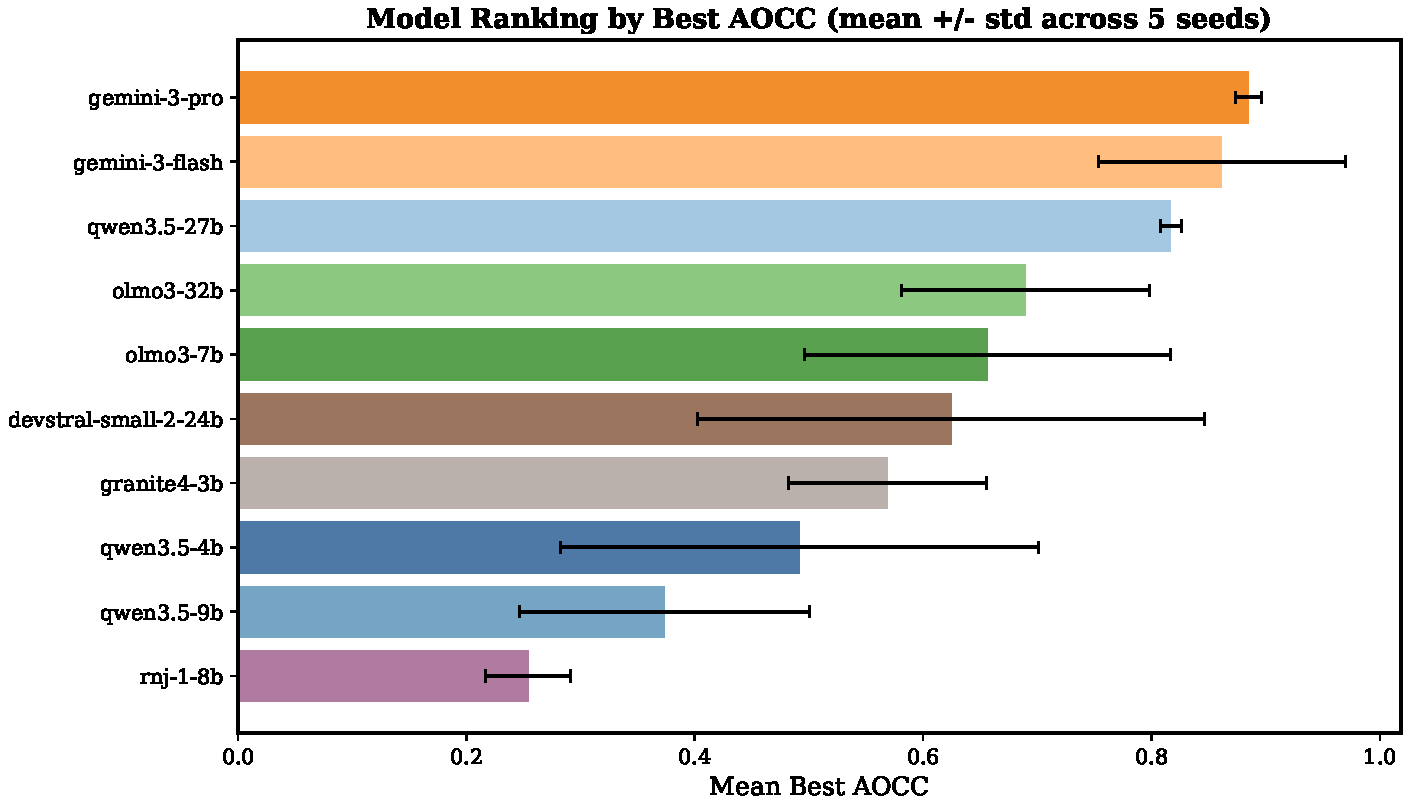
\includegraphics[width=\columnwidth]{figures/fig_model_ranking.pdf}
  \caption{Mean best AOCC by model ($\pm$ std across 5 seeds). API models (Gemini) dominate, while model size does not predict performance among local models.}
  \label{fig:model-ranking}
\end{figure}

The Kruskal--Wallis test confirms significant differences across models ($H = 38.6$, $p < 0.001$). Several patterns emerge:

\begin{itemize}
  \item \textbf{API models dominate.} Gemini~3 Pro achieves the highest mean best AOCC ($0.885 \pm 0.011$) with remarkable consistency (bootstrap 95\% CI: $[0.875, 0.893]$). Gemini~3 Flash is close behind ($0.862$) with the lowest failure rate ($2.0\%$).

  \item \textbf{Size does not predict quality.} Qwen3.5~27B ($0.817$) outperforms the larger OLMo~3 32B ($0.690$). Granite~4 at 3B ($0.569$) outperforms both Qwen3.5~9B ($0.373$) and RNJ-1~8B ($0.254$).

  \item \textbf{Failure rates vary dramatically}, from $2.0\%$ (Gemini~3 Flash) to $91.6\%$ (Qwen3.5~9B).
\end{itemize}

% Placeholder for convergence figure - export from notebook
\begin{figure}[t]
  \centering
  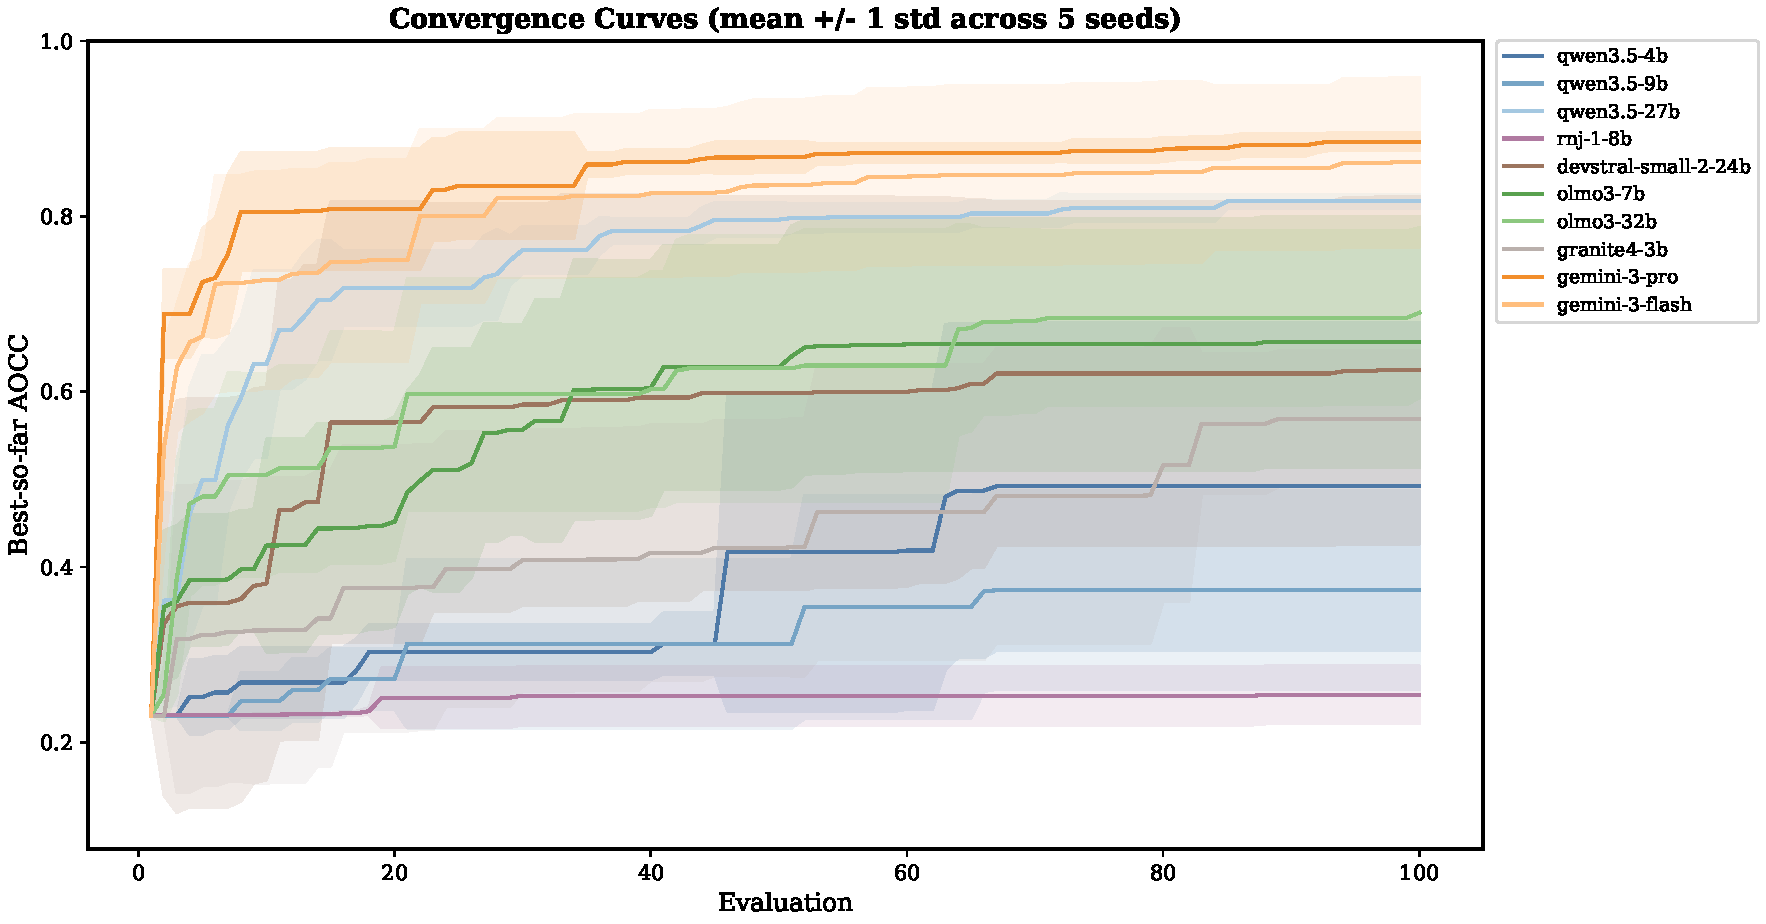
\includegraphics[width=\columnwidth]{figures/fig_model_convergence.pdf}
  \caption{Best-so-far AOCC over 100 evaluations for each model, averaged across 5 seeds. Shaded regions show $\pm$1 standard deviation.}
  \label{fig:model-convergence}
\end{figure}

\subsection{Failure Mode Analysis}
\label{sec:results-failures}

Across all 10 models and 5 seeds (5{,}000 total candidates), $3{,}071$ ($61.4\%$) produced valid fitness scores. Failures are dominated by runtime errors (logic bugs in generated code) for top models, and structural failures (producing functions instead of classes) for weaker models. RNJ-1 exhibits extreme failure burstiness: a $0.871$ probability of consecutive failure (vs.\ $0.074$ after a success), with a maximum streak of 81.

\begin{figure}[t]
  \centering
  
\includegraphics[width=\columnwidth]{figures/fig_failure_modes.pdf}
  \caption{Failure mode distribution by model. Categories: runtime errors (correct interface, logic bugs), structural failures (no class produced), and import errors.}
  \label{fig:failure-modes}
\end{figure}

\subsection{Model Selection}
\label{sec:results-model-selection}

\textbf{Gemini~3 Flash} is selected for Stage~3 based on its combination of competitive AOCC ($0.862$), lowest failure rate ($2.0\%$), and fast inference (3.9h/run). Its vanilla performance across 5 seeds ($0.862 \pm 0.097$) serves as the baseline for all Stage~3 comparisons.

The best algorithms reveal distinct model tendencies: Gemini produced CMA-ES variants (\texttt{BIP\_AMOS\_NES}, AOCC $= 0.923$), while open-weight models favoured Differential Evolution with local search. Code similarity confirms high diversity across models (mean pairwise similarity $= 0.061$).

% ===========================================================================
\section{Stage 2: Feature Analysis and Selection}
\label{sec:results-features}

The Stage~1 dataset contains $3{,}071$ valid candidates with behavioural feature vectors. None of the 32 features exhibited $>$50\% missing values.

\subsection{Feature--AOCC Correlations}
\label{sec:results-correlations}

\begin{figure}[t]
  \centering
  
\includegraphics[width=\columnwidth]{figures/fig_spearman_heatmap.pdf}
  \caption{Spearman rank correlation ($\rho$) between each behavioural feature and AOCC across all valid candidates. Features sorted by $|\rho|$.}
  \label{fig:spearman-heatmap}
\end{figure}

Spearman correlations (Bonferroni-corrected) reveal strong associations. The top-5 by $|\rho|$: \texttt{avg\_improvement} ($-0.782$), \texttt{step\_size\_autocorrelation} ($+0.766$), \texttt{improvement\_spatial\_correlation} ($+0.757$), \texttt{intensification\_ratio} ($+0.725$), and \texttt{fitness\_plateau\_fraction} ($+0.685$). All significant at $p < 0.001$. Notably, four of five are novel features from this thesis.

A Random Forest trained on all 32 features achieves OOB $R^2 = 0.962$, showing that behavioural features almost entirely determine AOCC.

\subsection{Consensus Ranking and Selection}
\label{sec:results-selection}

Three ranking methods (Spearman, RF importance, KS effect) are aggregated via Borda count. \Cref{tab:selected-features} shows the 10 features retained after greedy de-duplication ($|\rho| > 0.8$).

\begin{table}[t]
\centering
\caption{Selected features for Stage~3 (Borda consensus, $|\rho|>0.8$ de-duplication).}
\label{tab:selected-features}
\footnotesize
\begin{tabular}{@{}rlrr@{}}
\toprule
\textbf{\#} & \textbf{Feature} & \textbf{Src} & \boldmath{$\rho$} \\
\midrule
1  & avg\_improvement          & B & $-$.782 \\
2  & intensification\_ratio    & B & $+$.725 \\
3  & fitness\_plateau\_frac    & T & $+$.685 \\
4  & step\_size\_autocorr      & T & $+$.766 \\
5  & impr\_spatial\_corr       & T & $+$.757 \\
6  & half\_convergence\_time   & T & $-$.597 \\
7  & fitness\_autocorrelation  & T & $+$.645 \\
8  & x\_spread\_early          & T & $-$.599 \\
9  & longest\_no\_improv\_streak & B & $-$.469 \\
10 & dim\_conv\_heterogeneity  & T & $+$.471 \\
\bottomrule
\end{tabular}
\\[0.3em]
{\scriptsize B = BLADE~\cite{vanStein2025Behaviour}, T = This thesis.}
\end{table}

Three features come from BLADE, and seven are new. Seven redundant features were pruned (e.g., \texttt{success\_rate}, $|\rho|=0.917$ with \texttt{avg\_improvement}).

% ===========================================================================
\section{Stage 3: Behavioural Feedback}
\label{sec:results-feedback}

\subsection{Overall Format Comparison}
\label{sec:results-overall}

\begin{table}[t]
\centering
\caption{Overall performance by format (all 10 features pooled).}
\label{tab:format-overall}
\footnotesize
\begin{tabular}{@{}lrrr@{}}
\toprule
\textbf{Format} & \textbf{AOCC} & \textbf{Rank} & \textbf{Wins} \\
\midrule
Neutral     & 0.855 & 1.62 & 29/50 \\
Directional & 0.827 & 1.84 & 16/50 \\
Comparative & 0.784 & 2.49 & ~5/50 \\
\bottomrule
\end{tabular}
\end{table}

The Kruskal--Wallis test confirms a significant difference among formats ($p = 0.003$). Neutral dominates on all three metrics (\cref{tab:format-overall}). More prescriptive guidance correlates with worse performance.

Neutral conditions also have the \emph{highest} failure rate ($3.5\%$ vs.\ $2.6\%$ directional, $1.5\%$ comparative), suggesting neutral feedback encourages more ambitious algorithm designs.

\begin{figure}[t]
  \centering
  
\includegraphics[width=\columnwidth]{figures/fig_format_boxplot.pdf}
  \caption{Best AOCC distribution by feedback format across all features. Box: IQR; line: median; whiskers: 1.5$\times$IQR. Kruskal--Wallis $p = 0.003$.}
  \label{fig:format-boxplot}
\end{figure}

\subsection{Per-Condition Results}
\label{sec:results-conditions}

\Cref{tab:condition-ranking} and \cref{fig:condition-ranking} rank all 29 conditions. The top four are all neutral.

\begin{figure*}[t]
  \centering
  
\includegraphics[width=0.85\textwidth]{figures/fig_condition_ranking.pdf}
  \caption{All 29 conditions ranked by mean best AOCC ($\pm$ std, 5 seeds). Grey bar and dashed line show the vanilla baseline ($0.862$). Colours: blue = neutral, orange = directional, green = comparative.}
  \label{fig:condition-ranking}
\end{figure*} The second-ranked condition (\texttt{neutral-dim\_conv\_heterogeneity}, AOCC $= 0.905 \pm 0.006$) is a novel feature from this thesis (Borda rank 10), yet produces the second-best performance with the lowest variance of any condition.

\begin{table*}[t]
\centering
\caption{All 29 conditions ranked by mean best AOCC ($\pm$ std, 5 seeds). Vanilla baseline: $0.862 \pm 0.097$. Format: N = neutral, D = directional, C = comparative.}
\label{tab:condition-ranking}
\footnotesize
\begin{tabular}{@{}rlrr|rlrr|rlrr@{}}
\toprule
\# & \textbf{Condition} & \textbf{AOCC} & \textbf{F\%}
& \# & \textbf{Condition} & \textbf{AOCC} & \textbf{F\%}
& \# & \textbf{Condition} & \textbf{AOCC} & \textbf{F\%} \\
\midrule
1  & N-intens\_ratio  & .907$\pm$.021 & 4.2
& 11 & N-fitness\_autocorr & .841$\pm$.074 & 3.4
& 21 & D-x\_spread & .793$\pm$.109 & 3.2 \\
2  & N-dim\_conv\_het  & .905$\pm$.006 & 2.2
& 12 & D-fitness\_autocorr & .814$\pm$.068 & 1.0
& 22 & N-longest\_streak & .789$\pm$.109 & 2.6 \\
3  & N-plateau\_frac  & .891$\pm$.005 & 7.6
& 13 & C-plateau\_frac & .811$\pm$.077 & 1.4
& 23 & D-dim\_conv\_het & .788$\pm$.068 & 2.2 \\
4  & N-avg\_improv    & .883$\pm$.055 & 2.2
& 14 & N-step\_autocorr & .810$\pm$.111 & 1.8
& 24 & C-impr\_spatial & .786$\pm$.100 & 1.2 \\
5  & D-plateau\_frac  & .874$\pm$.055 & 3.0
& 15 & D-intens\_ratio & .806$\pm$.044 & 2.0
& 25 & C-dim\_conv\_het & .779$\pm$.072 & 2.8 \\
6  & D-avg\_improv    & .866$\pm$.060 & 3.4
& 16 & D-step\_autocorr & .798$\pm$.075 & 2.0
& 26 & C-step\_autocorr & .761$\pm$.103 & 0.8 \\
7  & D-half\_conv     & .862$\pm$.083 & 6.0
& 17 & C-avg\_improv & .860$\pm$.076 & 2.8
& 27 & C-half\_conv & .758$\pm$.060 & 0.6 \\
8  & D-longest\_streak & .860$\pm$.059 & 1.8
& 18 & C-x\_spread & .852$\pm$.092 & 1.8
& 28 & C-fitness\_autocorr & .750$\pm$.122 & 1.6 \\
9  & N-impr\_spatial  & .853$\pm$.089 & 1.8
& 19 & N-half\_conv & .847$\pm$.069 & 4.4
& 29 & C-intens\_ratio & .721$\pm$.046 & 0.6 \\
10 & D-impr\_spatial  & .857$\pm$.044 & 1.8
& 20 & N-x\_spread & .844$\pm$.067 & 4.4
&    &                 &               &     \\
\bottomrule
\end{tabular}
\end{table*}

The strongest format effect is on \texttt{intensification\_ratio}: neutral $0.907$ vs.\ comparative $0.721$ ($p = 0.002$, Cliff's $d = 1.0$). A second significant effect appears on \texttt{dim\_conv\_heterogeneity} ($p = 0.009$), where neutral ($0.905$) dramatically outperforms directional ($0.788$) and comparative ($0.779$). \Cref{fig:convergence-by-format} shows the convergence dynamics per feature and format.

\begin{figure*}[t]
  \centering
  
\includegraphics[width=\textwidth]{figures/fig_convergence_by_format.pdf}
  \caption{Best-so-far AOCC over 100 evaluations for each feature, split by feedback format (mean $\pm$ 1 std, 5 seeds). Neutral (blue) typically converges fastest and highest.}
  \label{fig:convergence-by-format}
\end{figure*}

\subsection{The Steering Paradox}
\label{sec:results-steering}

A natural hypothesis is that prescriptive feedback degrades performance because the advice is wrong. It is not. \Cref{tab:steering-accuracy} shows that for all five top features, the coded direction matches the empirical Spearman correlation.

\begin{table}[t]
\centering
\caption{Steering accuracy for top-5 features. Shift = median change vs.\ neutral. $\checkmark$ = correct direction, $\times$ = wrong.}
\label{tab:steering-accuracy}
\footnotesize
\begin{tabular}{@{}lrcc@{}}
\toprule
\textbf{Feature} & \textbf{Advice} & \textbf{Dir.} & \textbf{Comp.} \\
\midrule
avg\_improv   & Lower  & $+.012\;\times$ & $+.010\;\times$ \\
intens\_ratio & Higher & $-.030\;\times$ & $+.038\;\checkmark$ \\
plateau\_frac & Higher & $-.085\;\times$ & $+.105\;\checkmark$ \\
step\_autocorr & Higher & $-.034\;\times$ & $-.020\;\times$ \\
impr\_spatial  & Higher & $-.019\;\times$ & $-.020\;\times$ \\
\bottomrule
\end{tabular}
\end{table}

Directional feedback steers the wrong way for 5/5 top features. Across all 10 features, accuracy improves slightly: directional is correct for 3/10, comparative for 4/9, giving an overall accuracy of 7/19 (37\%). The advice is correct, but the LLM cannot translate it into appropriate code changes. This is the central empirical finding.

\subsection{AOCC-Matched Analysis}
\label{sec:results-aocc-matched}

To isolate the behavioural effect from performance differences, we compare feature distributions \emph{within} AOCC bands (low 0.3--0.5, mid 0.5--0.7, high 0.7--0.85, elite $>$0.85).

Of 19 testable feature $\times$ band combinations, \textbf{16 show significant differences} ($p < 0.05$), confirming the LLM produces behaviourally different code. But within-band steering accuracy is 9/19 (47\%) for directional and 8/19 (42\%) for comparative, both essentially random. Steering is not systematically wrong, just unreliable.

\begin{figure}[t]
  \centering
  
\includegraphics[width=\columnwidth]{figures/fig_steering_shifts.pdf}
  \caption{Median behavioural feature shift for directional and comparative formats relative to neutral. Green bars indicate correct steering direction, red bars indicate wrong direction.}
  \label{fig:steering-shifts}
\end{figure}

\texttt{fitness\_plateau\_fraction} is the most steerable feature (correct across all four bands). \texttt{step\_size\_autocorrelation} is the least steerable. \texttt{intensification\_ratio} shows quality-dependent behaviour: steering helps in low/mid bands but hurts in high bands.

\subsection{Neutral Feedback Produces Good Behavioural Profiles}
\label{sec:results-neutral-profiles}

\Cref{tab:profile-comparison} compares behavioural profiles by format against performance tiers.

\begin{table}[t]
\centering
\caption{Feature values by AOCC tier vs.\ feedback format.}
\label{tab:profile-comparison}
\footnotesize
\setlength{\tabcolsep}{3pt}
\begin{tabular}{@{}l|rrr|rrr@{}}
\toprule
& \multicolumn{3}{c|}{\textbf{Tier}} & \multicolumn{3}{c}{\textbf{Format}} \\
& \textbf{B25} & \textbf{M50} & \textbf{T25} & \textbf{N} & \textbf{D} & \textbf{C} \\
\midrule
avg\_imp    & .133 & .096 & .078 & .094 & .105 & .104 \\
int\_ratio  & .730 & .792 & .868 & .813 & .783 & .852 \\
plat\_frac  & .199 & .366 & .594 & .448 & .364 & .553 \\
ss\_autocorr & .845 & .881 & .900 & .897 & .863 & .877 \\
imp\_spat   & .622 & .630 & .683 & .649 & .630 & .629 \\
\bottomrule
\end{tabular}
\\[0.3em]
{\scriptsize B25/M50/T25 = bottom 25\%/middle 50\%/top 25\% by AOCC. N/D/C = neutral/directional/comparative.}
\end{table}

Neutral algorithms naturally sit between mid-50\% and top-25\% tiers on most features without explicit steering. Directional pulls toward or below mid-50\% on 4/5 features. Comparative is mixed: near top-25\% for \texttt{intensification\_ratio} and \texttt{fitness\_plateau\_fraction}, but worse on the other three. Neutral feedback lets evolutionary selection drive behavioural improvement, while prescriptive feedback creates a multi-objective tension that degrades performance.

\subsection{Comparison to Vanilla Baseline}
\label{sec:results-vs-vanilla}

\begin{table}[t]
\centering
\caption{Top conditions vs.\ vanilla ($0.862 \pm 0.097$).}
\label{tab:vs-vanilla}
\footnotesize
\begin{tabular}{@{}lrl@{}}
\toprule
\textbf{Condition} & \textbf{AOCC} & \boldmath{$p$} \\
\midrule
N-intens\_ratio    & .907 ($+$.046) & $>.09$ \\
N-dim\_conv\_het   & .905 ($+$.043) & $>.09$ \\
N-plateau\_frac    & .891 ($+$.030) & $>.09$ \\
\midrule
C-intens\_ratio    & .721 ($-$.140) & $<.05$ \\
\bottomrule
\end{tabular}
\end{table}

No neutral condition reaches significance with 5 seeds. However, \texttt{neutral-intensification\_ratio} ($0.907 \pm 0.021$) shows a consistent $+0.046$ delta with very low variance. The worst comparative condition significantly degrades performance ($-0.140$, $p < 0.05$). Neutral behavioural feedback is at worst harmless and at best mildly beneficial, while prescriptive feedback carries substantial downside risk.
